\subsection{Полнота}
    Введем основные определения.
    \begin{definition}
    \emph{Бинарным оператором} называется конечный вектор $\overline{f} = (f_1, ..., f_n)$, в котором каждая $f_j$ является функцией алгебры логики от n переменных $(j = \overline{1, n})$.
    \end{definition}
    
    \begin{definition}
    Бинарный оператор называется \emph{линейным}, если каждая его компонента является линейной. Соответсвенно, бинарный оператор называется \emph{нелинейным}, если хотя бы одна из его компонент является нелинейной.
    \end{definition}
    
    \begin{definition}
    \emph{Слоем} называется композиция линейной булевой функции  и нелинейного бинарного оператора. \emph{Входным слоем} будем называть вектор $\overline{X} = (x_1, ... x_n)\in \{0, 1\}^n$, а \emph{выходным} "--- вектор $\overline{Y} = (y_1, ... y_m)\in \{0, 1\}^m$.
    Линейную часть слоя назовем \emph{весовой функцией}. Она применяется ко всем выходам предыдущего слоя, включая входной слой.
    Нелинейный оператор назовем \emph{функцией активации}. В качестве нее можно использовать и тождественный оператор.
    \end{definition}
    
    \begin{definition}
    \emph{Нейронной сетью} называется композиция функций, каждая из которых является слоем.
    \end{definition}
    
    Обозначим класс бинарных нейронных сетей с линейной булевой весовой функцией и нелинейным бинарным оператором в роли функции активации через $\mathfrak{B}$. Параметром этого класса будет семейство функций активации $F$. Справедлив следующий результат, относящийся к проблеме полноты бинарной нейронной сети с такой архитектурой.
    
    \begin{theorem}
    Какое бы семейство функций активации $F$ мы не взяли, класс бинарных нейронных сетей $\mathfrak{B}$ будет полон в $P_2$.
    \end{theorem}
    \begin{proof}
    Так как класс булевых линейных функций является предполным, то достаточно хотя бы одной нелинейной функции, чтобы нейронная сеть могла порождать $P_2$. По определению нелинейного бинарного оператора такая функция будет существовать, что доказывает теорему.
    \end{proof}
    
    Рассмотрим вопрос существования полной бинарной нейросети с двумя слоями. Справедлива следующая теорема.
    
    \begin{theorem}
    Существует бинарная нейронная сеть класса $\mathfrak{B}$ с двумя слоями, которая полна в $P_2$.
    \end{theorem}
    
    \begin{proof}
    Построим бинарную нейронную сеть, реализующую СДНФ функции. Во входном слое подаётся вектор $\overline{X} = (x_1, ... x_n)\in \{0, 1\}^n$, на котором хотим получить вектор значений. В первом слое будет бинарный оператор, состоящий из конъюнкций, то есть $f^1 = (f^1_1, ..., f^1_{2^n})$ $\forall f^1_j = \wedge$, $j = \overline{1, 2^n}$. Весовая функция $g$ первого слоя следующего вида: 
    \begin{equation*}
    g(x) =
    \begin{cases}
    x, &\text{x входит в конъюнкцию без отрицания}\\
    1 \oplus x, &\text{x входит в конъюнкцию c отрицанием}
    \end{cases}
    \end{equation*}
    Она позволит получать отрицания переменных при передаче их в конъюнкцию. Во втором слое бинарный оператор, принимающий на вход все конъюнкции СДНФ и реализующий их дизъюнкцию, то есть $f^2 = \vee$. Таким образом, функции активации (конъюнкция, дизъюнкция) — нелинейны, а весовая (исключающее «или») — линейна, и мы сохраняем структуру слоя бинарной нейронной сети класса $\mathfrak{B}$ (Рис. 1).
    
    \begin{figure}[h]
    \begin{center}
    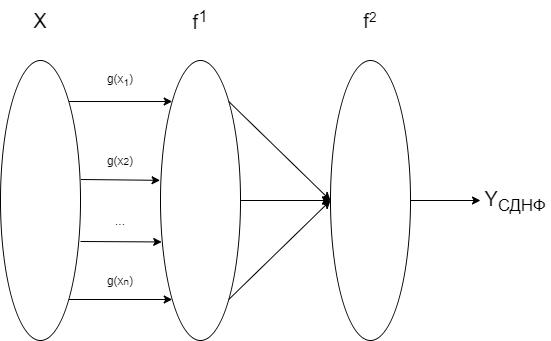
\includegraphics[width=1\linewidth]{picture1.png}
    \caption{}
    \label{ris:experimcoded}
    \end{center}
    \end{figure}
    
    Так как СДНФ функции конечна и единственна, то по ней мы сможем однозначно восстановить все функции алгебры логики, и такая нейронная сеть будет полна, что и требовалось доказать.
    \end{proof}
    
    Исторически, проблема выразимости нейронных сетей с вещественными значениями прослеживается от 13-й проблемы Гильберта, ставящей вопрос "существует ли непрерывная функция трех переменных, которая не может быть представлена через композицию непрерывных функций двух переменных". Она была решена в 1957 г. В.А. Арнольдом; oн показал, что любая непрерывная функция трех переменных представляется в виде композиции непрерывных функций двух переменных. В том же 1957 г. А.Н. Колмогоров доказал более сильную теорему: для реализации функций многих переменных достаточно операций суммирования и композиции функций одной переменной. Эта теорема в 1987 году была переложена Хехт–Нильсеном для нейронных сетей: любая функция нескольких переменных может быть представлена двухслойной нейронной сетью с прямыми полными связями с $N$ нейронами входного слоя, $(2N+1)$ нейронами скрытого слоя с ограниченными  функциями активации (например, сигмоидальными) и $M$ нейронами выходного слоя с неизвестными функциями активации \cite{seventh, eighth, ninth, tenth}.
    
    В бинарных нейронных сетях класса $\mathfrak{B}$ справедлив аналогичный результат.
    
    \begin{theorem}
    Какое бы семейство функций активации $F$ мы не взяли, класс бинарных нейронных сетей $\mathfrak{B}$ с четырьмя слоями будет полон в $P_2$.
    \end{theorem}
    
    \begin{proof}
    Из доказательства критерия Поста \cite{eleventh} известно, что имея нелинейную функцию, инвертор и константу 1, получим конъюнкцию. Имея конъюнкцию и инвертор, получим дизъюнкцию. Такая система будет полна. Среди линейных функций есть константа 1 и инвертор, в роли которого будет выступать исключающее «или» в виде $\overline{x} = 1 \oplus x$. Тогда на первом слое мы получим конъюнкцию, на втором — дизъюнкцию, а на третьем и четвертом — мы построим СДНФ нужной функции по \textbf{Теореме 2}.
    \end{proof}
    
    
\subsection{Аппроксимация}   
    В практике расчетов, связанных с обработкой экспериментальных данных, вычислением $f(x)$, разработкой вычислительных методов, встречаются следующие две ситуации:
    
    \begin{enumerate}
    \item Как установить вид функции $y = f(x)$, если она неизвестна? Предполагается при этом, что задана таблица ее значений, которая получена либо из экспериментальных измерений, либо из сложных расчетов.
    \item Как упростить вычисление известной функции $f(x)$ или же её характеристик, если $f(x)$ слишком сложная?
    \end{enumerate}
    
    Ответы на эти вопросы даются теорией аппроксимации функций, основная задача которой состоит в нахождении функции $\varphi(x)$, близкой (т.е. аппроксимирующей) в некотором нормированном пространстве к исходной функции $y = f(x)$. Функцию $\varphi(x)$ при этом выбирают такой, чтобы она была максимально удобной для последующих расчетов.
    
    Одним из замечательных свойств нейронных сетей с вещественными значениями является способность аппроксимировать и, более того, быть универсальными аппроксиматорами. С их помощью можно аппроксимировать сколь угодно точно непрерывные функции многих переменных. \cite{twelfth}
    
    Что касается бинарных нейронных сетей, здесь этот вопрос ещё хорошо не изучен. Важно доказать, насколько хорошо можно аппроксимировать любую булеву функцию линейными, то есть важен вопрос линейной аппроксимации в бинарном случае.
    
    \begin{definition}
    Пусть $f$ — булева функция от $n$ переменных, то есть $f: V^n \rightarrow \{0, 1\}$, где $V^n$ "--- булевый вектор размерности $n$. Ее \emph{весом} $w(f)$ будем называть количество наборов, на которых функция принимает значение 1.
    \end{definition}
    
    \begin{definition}
    Пусть $f, g$ — булевы функции от $n$ переменных. \emph{Расстоянием} от булевой функции $f$ до булевой функции $g$ называется величина $$dist(f, g) = w(f \oplus g),$$ то есть количество наборов, на которых значения $f$ и $g$ различаются. Расстоянием от $f$ до множества $M$ булевых функций от $n$ переменных назовем величину $$dist(f, M) = \min_{g \in M}\ dist(f, g).$$
    \end{definition}
    
    %Скажем, что булева функция $f$ \emph{близка} к булевой функции $g$, если расстояние $dist(f, g)$ между ними меньше некоторого фиксированного числа $\varepsilon$. В противном случае скажем, что булева функция $f$ \emph{далека} от булевой функции $g$. Аналогично и для расстояния между функцией $f$ и множества $M$.
    
    \textbf{Гипотеза.}
    Всегда найдется булева функция $f$ из класса нелинейных функций такая, что расстояние от нее до класса линейных будет больше числа $k \in \mathbb {N}$, то есть $dist(f, L) > k$.
    
    \textbf{Задача.}
    Найти максимальное число $k$, при котором гипотеза будет верна.
    
    \emph{Основная идея.}
    Известно, что линейных булевых функций от $n$ переменных $2^{n+1}$, а нелинейных "--- $2^{2^n} - 2^{n+1}$. То есть при $n \geqslant 3$ количество нелинейных функций начинает преобладать над количеством линейных.
    Необходимо рассмотреть систему шаров радиусами $k$, центрами которых будут линейные функциии. Внутри этих шаров будут нелинейные функции. Начиная с $k = 1$, увеличивать значение радиусов шаров на 1, пока все нелинейные функции не попадут в них. Итоговый радиус и будет порогом, когда линейные функции получают способность аппроксимировать нелинейные.
    
    Получив значение $k$, мы определим, насколько далеки нелинейные булевы функции от линейных. 